\documentclass[xcolor=dvipsnames]{beamer}
%\documentclass[t,handout]{beamer}
\usepackage{comment}
\usepackage{relsize}
\usepackage{pifont}
\usepackage{tipa, vowel}
%\usepackage{relsize}
\usepackage[english]{babel}
%\usepackage[latin1]{inputenc}
\usepackage{amsmath}
\usepackage{amsfonts}
\usepackage{amssymb}
\usepackage{fancyhdr}
%\usepackage[T1]{fontenc}
%\usepackage[pdftex]{graphicx}
\usepackage{multimedia}
\usepackage{hyperref}
\usepackage{xcolor}
\usepackage{graphics}
\usepackage[english,cleanlook]{isodate}

\newcommand{\YEAR}{\the\year}
\newcommand{\MONTH}{\the\month}

%%%%%%%%%%%%%%%%%%%%%%%%%%%%%%%%%%%%%%%%%%%%%%%%%%%%%%%%%%%%
%Presentation Themes
%%%%%%%%%%%%%%%%%%%%%%%%%%%%%%%%%%%%%%%%%%%%%%%%%%%%%%%%%%%%

%%%% no navigation bars:
%\usetheme{Bergen} %based on inmargin and rectangles
%\usetheme[secheader]{Boadilla} %much information on little space, option secheader gives current sections and subsection
%\usetheme{Pittsburgh}% alleen standaard nav
%\usetheme{Rochester}% helder, alleen standaard nav option [height] sets hight of frame title bar

%%%% tree-like  navigation bars:
%\usetheme{Antibes} %heel kaal
%\usetheme{JuanLesPins}
%\usetheme{Montpellier} % matig

%%%% table of contents sidebar:
%\usetheme{Berkeley}
%\usetheme[right,hideothersubsections]{PaloAlto}% nav links
%\usetheme[hideothersubsections]{Goettingen} % overzicht rechts
%\usetheme[hideothersubsections]{Marburg} % donkere navigatiebalk rechts
%\usetheme[right,hideothersubsections]{Hannover} % als Goetngen met overzicht links

%%%% mini frame navigation:
%\usetheme{Berlin}
%\usetheme{Dresden} %nice
%\usetheme{Ilmenau}
%\usetheme{Darmstadt}
%\usetheme{Frankfurt} %ok
%\usetheme{Singapore} %helder ok nav boven+#sheets indicatie
%\usetheme{Szeged} %helder ok nav boven+#sheets indicatie

%%%%section and subsection tables:
%\usetheme{Copenhagen}
%\usetheme{Luebeck} % overzicht boven, auteur beneden
%\usetheme{Malmoe} % nav boven
%\usetheme[]{Warsaw}

\usetheme[secheader]{Madrid} % alleen navigatie onder


%%%%%innerthemes: title and part pages, itemize, enumerate, desciption, block, theorem/proof, figures, tables, footnotes and bibl. entries 
%\useinnertheme{default} %
%\useinnertheme{circles} % 
%\useinnertheme{rectangles} %
\useinnertheme{rounded} %
%\useinnertheme{inmargin} %structure on left (like blocktitles) and normal info like block bodies on right

%%%%%outerthemes: head and footline, sidebars, logo, frame title
%\useoutertheme{infolines}%
%\useoutertheme[footline=authorinstituretitle, subsection=false]{miniframes}%
%\useoutertheme{smoothbars}%
%\useoutertheme[right,height=0pt,hideothersubsections]{sidebar}%options:height=dimension, hideothersubsections, hideallsubsections, left, right, width=dimension
%\useoutertheme{split}%
%\useoutertheme{shadow}%
%\useoutertheme{tree}%option:[hooks]
%\useoutertheme{smoothtree}%

%%%%%%%%%%%%%%%%%%%%%%%%%%%%%%%%%%%%%%%%%%%%%%%%%%%%%%%%%%%%
%Transparency Effects
%%%%%%%%%%%%%%%%%%%%%%%%%%%%%%%%%%%%%%%%%%%%%%%%%%%%%%%%%%%%
\setbeamercovered{transparent}

%%%%%%%%%%%%%%%%%%%%%%%%%%%%%%%%%%%%%%%%%%%%%%%%%%%%%%%%%%%%
%Color Themes:
%%%%%%%%%%%%%%%%%%%%%%%%%%%%%%%%%%%%%%%%%%%%%%%%%%%%%%%%%%%%
\usecolortheme{sidebartab} %highlights current entry in table of contents
%\usecolortheme[RGB={25,25,112}]{structure} %72,61,139
\usecolortheme[RGB={72,61,139}]{structure} %72,61,139

%%%%%%%%%
%\usecolourtheme [option]{structure} %options: rgb={} or RGB={} sets structure foreground colour
\usecolortheme{rose}
\usecolortheme{dolphin}

%\setbeamercolor{alerted text}{fg=red}
%\usecolortheme{sidebartab} %highlights current entry in table of contents
%\usecolortheme[RGB={25,25,112}]{structure} %72,61,139
%\usecolortheme[RGB={25,25,112}]{structure} %72,61,139
%\usecolortheme[RGB={39,64,139}]{structure}

%\usecolortheme[RGB={176,48,96}]{alerted text}

%%%%%%%innercolorthemes: changes palette colors
%\usecolortheme{lily} %used to restore default colours 
%\usecolortheme{orchid}
%\usecolortheme{rose}

%%%%%%%outercolourthemes:
%\usecolortheme{dolphin}
%\usecolortheme{whale}
%\usecolortheme{seahorse}

%%%%%%complete colorthemes:
%\usecolortheme{albatross}
%\usecolortheme{overlystylish}
%\usecolortheme{beetle}
%\usecolortheme{crane}
%\usecolortheme{dove}
%\usecolortheme{fly}
%\usecolortheme{seagull}

\setbeamercolor{frametitle}{bg=structure.fg!10!white,fg=structure.fg!10!black}
\setbeamercolor{block title}{fg=structure.fg!10!black}
\setbeamercolor{box}{bg=white}

%\setbeamercolor{outline}{fg=structure}
\setbeamercolor{sidebar}{bg=structure.fg!50!white}
\setbeamercolor{section in sidebar}{fg=structure}
\setbeamercolor{subsection in sidebar}{fg=structure}
\setbeamercolor{subsection in sidebar}{fg=structure}
\setbeamercolor{alerted text}{fg=purple}

\setbeamertemplate{bibliography item}{\insertbiblabel}

\title[Open Corpora and Privacy]{Open Corpora and Privacy Law}

\makeatletter
\def\name#1{\gdef\@name{#1\\}}
\makeatother
\author[van Son]{\em Rob van Son}

\institute[NKI-AVL]{{\normalsize Netherlands Cancer Institute, Amsterdam, The Netherlands}\\
	{\small R.v.Son@nki.nl}}
\date[\MONTH-\YEAR]{\today}


% Delete this, if you do not want the table of contents to pop up at
% the beginning of each subsection:
\begin{comment}

\AtBeginSection[] %or \AtBeginSubsecton{} 
{
  \begin{frame}<beamer>
    \frametitle{Outline}
    \tableofcontents[currentsection,currentsubsection,hideothersubsections]
  \end{frame}
}
\end{comment}


\begin{document}

\frame{\titlepage
	\parbox{0.33\textwidth}{
	\begin{center}
	\begin{figure}
	{
\includegraphics[width=0.30\textwidth]{Pictures/logo_ENG_Netherlands_Cancer_Institute_grootformaat}}
	\end{figure}
	\end{center}
	}
	\parbox{0.32\textwidth}{
	~
	}	
	\parbox{0.33\textwidth}{
	\begin{center}
	\begin{figure}
	{
\includegraphics[width=0.30\textwidth]{Pictures/aclc-logo}}
	\end{figure}
	\end{center}
	}
}

% \section*{Outline}
% 
% 	\frame{
% 	\frametitle{Outline}
% 	\tableofcontents[hidesubsections] %[pausesections]
% 	}

\section{Introduction}

\begin{frame}
	\frametitle{\insertsection}
		
	\begin{center}
	\begin{figure}[l]
     
\includegraphics[width=0.60\textwidth]{Pictures/Introduction}
	\end{figure}
	\end{center}
\end{frame}

\begin{frame}
	\frametitle{Two trends in science: Open Data and Privacy Protection}
	
	\begin{block}{Why Open Data?}
	\begin{itemize}
	\item Transparancy and trust
	\item Releasing scientific and social/commercial value of data
	\item Participation and Engagement
	\end{itemize}
\end{block}

\begin{block}{But there are privacy risks}
	\begin{itemize}
	\item Re-identification  \hspace{2.5cm}{\em speaker identification, MRI ``picture''}
	\item Combining of data sources \hspace{2.5cm}{\em health data \& shopping list}
	\item Social media, profiling, discrimination  \hspace{1.5cm}{\em bullying, pricing, work}
	\end{itemize}
	\end{block}
	
\end{frame}
	
\begin{frame}[label=Knowledge]
	\frametitle{Knowledge = Power}
	\begin{block}{Big Data}
	\begin{itemize}
	\item There have never been more data
	\item Big data revolutionizes technology
	\item Personalized health
	\item Machine learning allows effective AI
	\end{itemize}
	\end{block}
	
	\begin{block}{Asymmetric results}
	\begin{itemize}
	\item The Matthew effect: the strong get stronger, the weak get weaker
	\item Data is used {\em against} data subjects
	\item No trickle-down effect: the benefits stay mostly at the top
	\item Without privacy, no democracy
	\end{itemize}
	\end{block}
	\hyperlink{Intervention of the law}{The law steps in}
\end{frame}
	
	
\begin{frame}
	\frametitle{Intervention of the law}
	\begin{block}{The answer of the EU is the {\em General Data Protection Regulation}}
	\begin{itemize}
	\item Takes effect 25th May 2018
	\item Uniform\footnote[frame]{There is some variation at the national level} Data Protection law in the EU/single market
	\item Shifts balance of power to data subjects
	\item Technological and procedural fixes: {\em Privacy by Design}
	\item Designed to enforce compliance
	\end{itemize}
	\end{block}
	
	\begin{block}{Targeted at companies and big data, but:}
	\begin{itemize}
	\item Science is collateral damage, patched with exceptions (derogations)
	\item Paternalism could be devastating to (health) research
	\item Big data can be harmful without ``breaking'' privacy 
	\end{itemize}
	\end{block}
\end{frame}
	
\section{Corpora}
{\usebackgroundtemplate{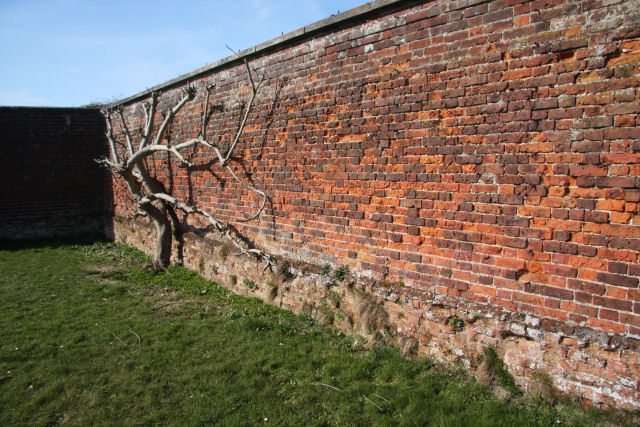
\includegraphics[width=\paperwidth]{Pictures/brick_wall}}
\begin{frame}
	\frametitle{\insertsection}
	
	\vskip 0.8cm
	
	\begin{figure}[l]
     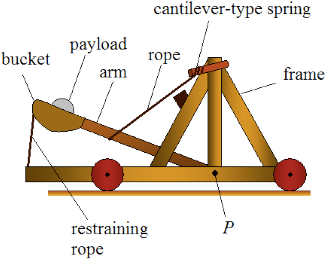
\includegraphics[width=0.60\textwidth]{Pictures/throw_over_the_wall2} \hspace{4cm}
	\end{figure}
	\begin{center}
	{\large Corpus construction}
	\end{center}
\end{frame}
}

\begin{frame}
	\frametitle{Data collection}
	Example: Speech corpus with added data on subjects (MRI, health data)
	
	\begin{block}{Workflow \footnote[frame]{This list can fill a workshop of its own {\scriptsize\cite{BestPractices2012}}} \hspace{7.5cm}{\em use standards!}}
	\begin{itemize}
	\item Formulate aims, target audience, and data management plan
	\item Compile informed consent and copyright transfer forms
	\item Approval from Research/Medical Ethical Committee  
	\item Recruit subjects
	\item Collection of raw recordings, and other data {\scriptsize\cite{draxler2012using}}
	\item Code all identifying data (pseudonymization)
	\item Select final data: segment recordings, add annotations etc. {\scriptsize\cite{drude2012best}}
	\item Compile metadata {\scriptsize\cite{CMDI}} and technical documentation
	\end{itemize}
	\end{block}

\end{frame}
	
\begin{frame}
	\frametitle{A corpus contains primary and secondary materials}
	
	\begin{block}{Primary materials: immutable or audit trail \hspace{2cm}{\em version control}}
	\begin{itemize}
	\item All recordings of subjects and all human annotations
	\item Data obtained from subjects, e.g., MRI, questionnaires
	\item Metadata and other subject data
	\item Technical documentation: how was the data collected (+scripts)
	\end{itemize}
	\end{block}
	If it requires human intervention $\Rightarrow$ primary data
	
	\begin{block}{Secondary materials}
	\begin{itemize}
	\item Everything that can be derived from the primary data
	\item Scripts used to generate secondary data
	\item Documentation \& Publications
	\end{itemize}
	\end{block}
	If it is generated automatically $\Rightarrow$ secondary data
\end{frame}

\begin{frame}
	\frametitle{Points of attention}
	\begin{block}{Keep in mind}
	\begin{itemize}
	\item {\color{Maroon} The informed consent limits what can be done with a corpus}
	\item {\color{Maroon} ``Speech'' is published: collect copyright transfers from {\em all} involved}
	\item Keep contact data far, far away from corpus data
	\item Code (pseudonymize) subject id's at the earliest possible moment
	\item A corpus is useless without metadata and documentation
	\item Filenames should be unique and descriptive (speakers, task, lang., ...)
	\item A lot of data is privacy sensitive, keep it under lock and key\\
		(no public cloud storage or insecure file transfer!)
	\end{itemize}
	\end{block}
\end{frame}

\begin{frame}
	\frametitle{More information}
	LREC2012: Best Practices for Speech Corpora in Linguistic Research {\scriptsize\cite{BestPractices2012}}\\
	Especially:
	\begin{itemize}
	\item \cite{draxler2012using} Using A Global Corpus Data Model for Linguistic and Phonetic Research  
	\item \cite{drude2012best} Best practices in the design, creation and dissemination of speech corpora at The Language Archive
	\item \cite{macwhinney2012best} Best Practices in the TalkBank Framework
	\item \cite{cieri2012toward} Toward the Harmonization of Metadata Practice for Spoken Languages Resources
	\end{itemize}
	See also:
	\begin{itemize}
	\item \cite{hart2016ten} Ten Simple Rules for Digital Data Storage
	\end{itemize}
	\nocite{vanson2017notes}
\end{frame}

\section{GDPR}
\begin{frame}
	\frametitle{\insertsection - General Data Protection Regulation}
	
	\begin{center}
	\begin{figure}
	{
\includegraphics[width=0.90\textwidth]{Pictures/DragonAttack}}
	\end{figure}
	The GDPR and Big Data
	\end{center}
	\let\thefootnote\relax\footnotetext{\hspace{-16.5pt}\scriptsize \em Disclaimer: the author is not a lawyer and this is not legal advice}
\end{frame}


\begin{frame}[label=Accountability]
	\frametitle{Accountability: demonstration of compliance}
	
	\begin{block}{Bullet points to consider when building a corpus}
	\begin{itemize}
	\item Privacy Impact Assessment (PIA)
	\item Privacy by Design technology
	\item Approvals from the Research/Medical Ethical Committee (R/MEC)
	\item Approval from the Data Protection or Privacy Officer (DPO/PO)
	\item Collect explicit, written informed consents and copyright transfers
	\vskip 0.5cm
	\item If there is protected content, collect legally binding
	\begin{itemize}
	\item Promise of Confidentiality (PoC)
	\item Non Disclosure Agreements (NDA)
	\item Data Transfer Agreements (DTA)
	\end{itemize}
	\item If necessary, vet the credentials of the recipients
	\end{itemize}
	\end{block}	

\end{frame}

\begin{frame}
	\frametitle{Privacy Impact Assessment (PIA)}
	
	\begin{block}{Risk/benefit assessment of the corpus {\hspace{4.5cm}\scriptsize\cite{act2014conducting,Art29DPWP}}}
	\begin{itemize}
	\item Why\footnote[frame]{This bullet is not strictly a part of a PIA, but you need it anyway} is the data important? What are the benefits to society?
	\item The impact of data exposure on the data subjects?
	\item What is done to reduce the impact of data exposure?
	\item The risks to the data? List them
	\item What is done to reduce the risk of data exposure?
	\item Procedures to ensure policies are complied with
	\item Procedures to notify authorities and subjects of a data breach
	\item Procedures, if any, to honor retractions of consent (backups!)
	\end{itemize}
	\end{block}	
	
\end{frame}

\begin{frame}
	\frametitle{Privacy by design}
	
	\begin{block}{Technology and policy ``suggestions'' in the GDPR {\hspace{1cm}\scriptsize\cite{IAPP2016Top10,AnitaVocht2016,AllenOvery2016GDPR,ico2017Overview}}}
	\begin{itemize}
	\item Data minimization {\hspace{2cm} \small \em what is not there, cannot be exposed}
	\begin{itemize}
	\item Coarse-graining: age-brackets, truncate zip codes, etc.
	\item Strip metadata from images, movies, MRI
	\item Censor bars in pictures, movies, MRI 
	\end{itemize}
	\item Anonymization {\hspace{2.6cm} \small \em if data is useful, it is not anonymous}
	\item Pseudonymization
	\item Encryption
	\item Security, computer and otherwise
	\item Procedures, policies, codes of conduct, certification
	\item Other: Take the analysis to the data {\scriptsize\cite{budin2015datashield}}
	\end{itemize}
	\end{block}	

	When used, these must be fully documented (PIA)

\end{frame}

\begin{frame}[label=Approvals]
	\frametitle{Approvals of REC/MEC \& DPO/PO}
	
	\begin{block}{Get approval, needed are:}
	\begin{itemize}
	\item Protocols
	\item Informed consent and copyright transfer forms
	\item The results of the PIA
	\item Data management plan {\scriptsize\cite{AcademyFinland20DMP}}
	\item Secure storage and dissemination (technology)
	\item NDA or DTA papers when relevant
	\item Whatever more is requested by the committees or officers
	\end{itemize}
	\end{block}	
\end{frame}

\begin{frame}[label=Informed consent and copyright transfers]
	\frametitle{Informed consent and copyright transfers}
	
	\begin{block}{\hyperlink{Clinical Trial Informed Consent}{Be specific {\em and} open ended {\hspace{6.5cm} \scriptsize $>$}}}
	\begin{itemize}
	\item \hyperlink{Clinical Trial Informed Consent}{Informed consent is a process to enable a subject to make an {\em enlightened decision} to participate or not ({\em Nuremberg Code, 1947}})
	\item \hyperlink{Clinical Trial Informed Consent}{Extensive rules for Informed Consent\footnote[frame]{Consent rules for health data differ between EU member states}, cf. GCP {\scriptsize\cite{ICH1996GCP}}}
	\item Currently unclear how specific consent must be
	\item Procedures for retraction of consent and requests for information
	\vskip 0.5cm
	\item Who will receive the copyrights to the corpus?
	\item Everyone involved in the corpus must also transfer her/his copyrights
	\item Store all signed paper forms, not just scanned images
	\vskip 0.5cm
	\item Note that this paperwork determines how useful the data will be!
	\end{itemize}
	\end{block}	
\end{frame}

\begin{frame}
	\frametitle{Binding restrictions on use}
	{\em When information is protected}
	\begin{block}{DTAs, NDAs, or PoC}
	\begin{itemize}
	\item Sharing only possible with legally binding restrictions on use
	\item Not every researcher can guarantee the required confidentiality
	\item Recipient institutions must be qualified
	\item Some uses \& users require new ethical (R/MEC) approval
	\item Consider to split the corpus and allow access to a ``free-ish'' subset
	\item Set up platform to perform sensitive processing in-house {\scriptsize\cite{budin2015datashield}}\\
			{\em Take the analysis to the data {\scriptsize\cite{DataSHIELD2014:short}}}
	\end{itemize}
	\end{block}	
\end{frame}

\begin{frame}
	\frametitle{Problems}
	
	\begin{block}{Open questions}
	\begin{itemize}
	\item GDPR $\Leftrightarrow$ Clinical Trials Regulation (CTR) {\scriptsize\cite{dittrich2015esmod}}
	\item EU vs. National rules on health data and consent (CTR, {\scriptsize\cite{chassang2017impact}})
	\item What health data fall under the research derogation, if any?
	\item Consent must be specific, but the use of open data is not
	\item What research is ``in the public interest''?
	\item Open data is international, the GDPR restricts cross-border exchange
	\item Do rights of data subjects apply to open data?
	\begin{itemize}
	\item retract consent, right to be forgotten
	\item be informed about use
	\item be informed about export to other countries
	\end{itemize}
	\item Can Open Data be squared with NDAs and DTAs? Is it necessary?
	\end{itemize}
	\end{block}	
\end{frame}


\begin{frame}
	\frametitle{Solutions \hspace{6.7cm}{\em do they exist?}}
	
	\begin{block}{How can these problems be approached}
	\begin{itemize}
	\item {\color{OliveGreen} Write sensible informed consent forms}
	\item {\color{OliveGreen} Partition corpora into unprotected and protected parts}
	\item {\color{OliveGreen} Publish aggregate data and (truly) anonymous derived data}
	\item {\color{OliveGreen} Perform data analysis in-house and only export results {\scriptsize\cite{budin2015datashield}}}
	\item {\color{MidnightBlue} Formulate guidelines, cf. {\em Good Clinical Practice} (GCP)}
	\item {\color{MidnightBlue} Formulate guidance on data subject rights}
	\item {\color{MidnightBlue} Guidelines on what research data are subject to what rules}
	\item {\color{Maroon} Harmonize rules in EU on health data and consent (CTR?)}
	\item {\color{Maroon} Recognize autonomy of data subjects in consent rules}
	\item {\color{Maroon} Recognize the right to be altruistic and to participate in research}
	\end{itemize}
	\end{block}	
\end{frame}

\section{Conclusions}
\begin{frame}
	\frametitle{\insertsection}
	
	\begin{center}
	\begin{figure}
	{
\includegraphics[height=0.60\textheight]{Pictures/Riding_into_the_sunset}
	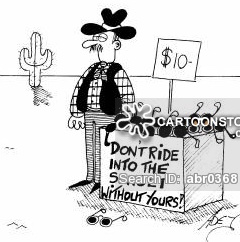
\includegraphics[height=0.50\textheight]{Pictures/Riding_into_the_sunset2}}
	\end{figure}
	
	\end{center}
\end{frame}

\begin{frame}
	\frametitle{Concluding remarks}
	
	\begin{block}{Informed Consent is central}
	\begin{itemize}
	\item In theory, anything should be possible with the right Informed Consent
	\item However, in practice
		\begin{itemize}
		\item R/MEC will limit what can be asked from subjects
		\item A valid Informed consent must be specific and cannot be open ended\footnote[frame]{Might vary between EU member states, CTR}
		\item [$>$]{\color{Maroon} But, a TV reality show can broadcast any health data about a person}
		\end{itemize}
	\item Autonomous citizens $\Leftrightarrow$ legal protections of the GDPR?
	\end{itemize}
	\end{block}
	
	\begin{block}{For protected data}
	\begin{itemize}
	\item Become competent and only share with competent parties
	\item Guidelines for the handling of research data (e.g., {\em GCP})
	\item GDPR prefers binding Codes of Conduct and Certification
	\item Bring analysis to the data
	\end{itemize}
	\end{block}

\end{frame}

\begin{frame}
	\begin{center}
	To be continued...\\
	~\\~\\
	{\Huge Thank You!}\\
	~\\~\\
	\resizebox{0.1\linewidth}{!}{?}
	\end{center}
\end{frame}

\begin{frame}[allowframebreaks]
        \frametitle{More information}
\bibliographystyle{ieeetr}
\begin{scriptsize}
\bibliography{NotesOnCorpusConstruction}
\end{scriptsize}

\vskip 0.5cm
\begin{center}

\includegraphics[width=0.3\textwidth]{Pictures/CC-share-alike}\\
{\small This work is licensed under a Creative Commons Attribution-ShareAlike 4.0 International License.}\\
\copyright {\YEAR}  R.J.J.H. van Son
\end{center}

\end{frame}

\appendix

\section{Clinical Trial Informed Consent}

\begin{frame}[label=Clinical Trial Informed Consent]
	\frametitle{\insertsection}
	
	\begin{center}
	\begin{figure}
	{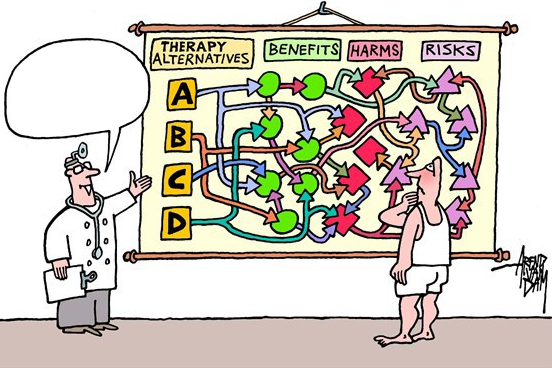
\includegraphics[height=0.80\textheight]{Pictures/InformedConsent}}
	\end{figure}
	\end{center}
\end{frame}


\begin{frame}
	\frametitle{\insertsection ~ {\scriptsize\cite{informedconsentWHO,dittrich2015esmod}}}
	
	A process by which a subject {\bf voluntarily} confirms his or her willingness to participate 
	in  a  particular  trial,  after  having  been  {\bf informed  of  all  aspects  of  the  
	trial}  that  are relevant  to  the  subject's  decision  to  participate.  Informed  
	consent  is  {\bf documented  by means of a written, signed and dated} informed consent form.
	
	\hspace{9cm}{\em ICH GCP 1.28}
	\vskip 0.5cm
	
\end{frame}

\begin{frame}
	\frametitle{Subject information}

	\begin{block}{Informed Consent discussion and written information}
	\begin{itemize}
	\item Ethical Principles, Dec. of Helsinki
	\item Required elements of ICH GCP 4.8.10 (20 elements) {\scriptsize\cite{ICH1996GCP}}
	\end{itemize}
	\end{block}	
	
	\begin{block}{Subject Information Sheet}
	\begin{itemize}
	\item Highly controlled document
	\item Approved by a Recognised Ethical Committee
	\item Authorisation of Institutional Medical Board
	\item Roles:
	\begin{itemize}
		\item Investigator: Communicate and Explain
		\item Subject: Assess and make informed decision
	\end{itemize}
	\end{itemize}
	\end{block}	
\end{frame}

\begin{frame}
	\frametitle{Subjects}

	\begin{block}{Important considerations}
	\begin{itemize}
	\item {\em No} advertisement or recruitment before approval (EC\&IMB)
	\item {\em No} study specific procedures performed before signed consent  
	\item Consented Subjects:
	\begin{itemize}
		\item Copy of Subject Information Sheet
		\item Inform General Practitioner if Subject agreed
	\end{itemize}
	\item Inform Subjects of any developments relevant to consent
	\item Keep all written documents {\em (not just scans)}
	\end{itemize}
	\end{block}
	
\end{frame}

\begin{frame}
	\frametitle{Process}

	\begin{block}{Informed Consent discussion}
	\begin{itemize}
	\item Interview with investigator required (or other staff)
	\item Investigator  
	\begin{itemize}
		\item Assure Subject understood all information
		\item Assure all questions have been answered
		\item Obtain voluntary written informed consent
	\end{itemize}
	\item Minors and incapacitated adults
	\begin{itemize}
		\item Discussion involves every person with parental/legal responsibility\\
			(incapacitated adults) Person unconnected to the trial
		\item Information is presented to capacity of Subject
		\item Assent: explicit wish of subject is considered
	\end{itemize}
	\item Informed consent {\color{Maroon}signed} and {\color{Maroon}dated} by Subject {\color{Maroon}\em and} Investigator
	\end{itemize}
	\end{block}
	
\end{frame}


\begin{frame}
	\frametitle{Example Minimal Informed Consent form {\scriptsize\cite{informedconsentutwente}}}

	\begin{center}
	\vskip -1.4cm
	\begin{figure}
	\href{https://www.utwente.nl/en/bms/research/forms-and-downloads/example-informed-consent-form.pdf}
	{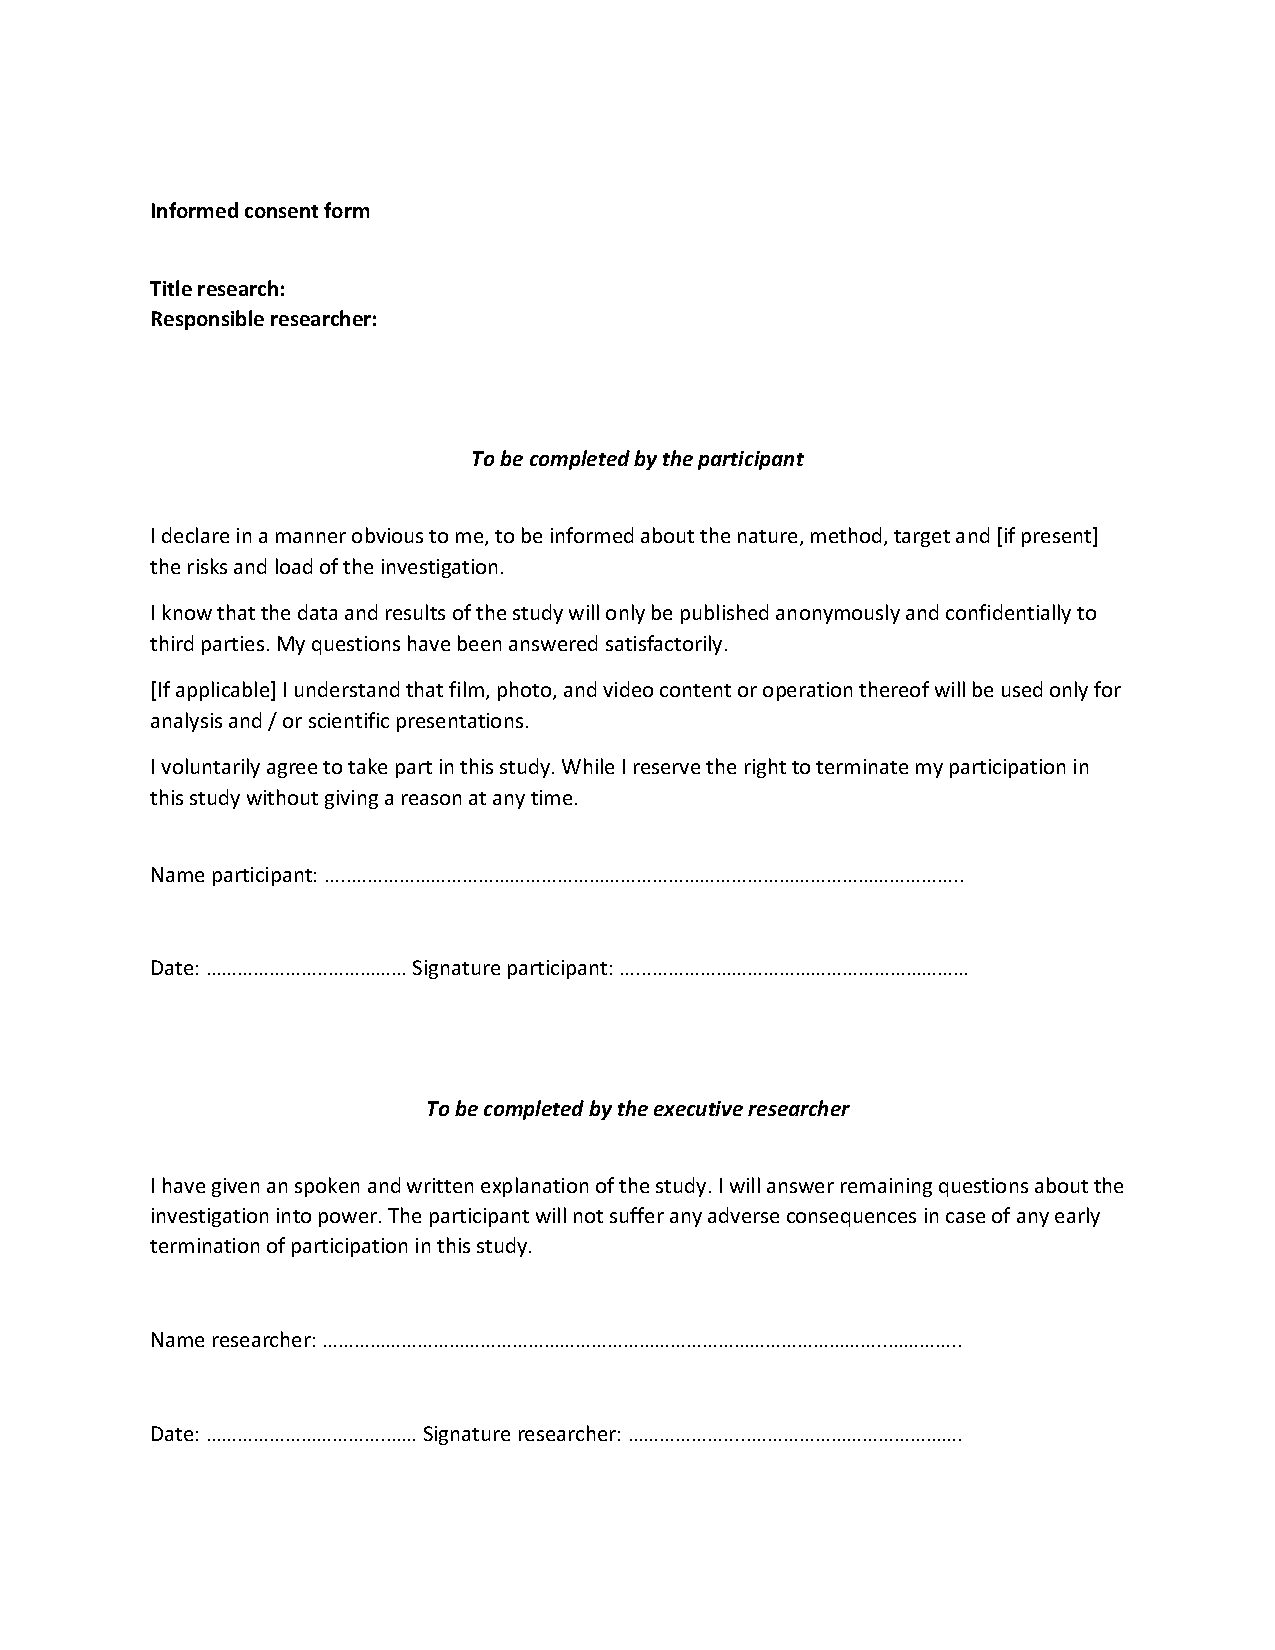
\includegraphics[height=1.1\textheight]{Pictures/example-informed-consent-form}}
	\end{figure}
	\end{center}

\end{frame}

\begin{frame}
	\frametitle{Information sheet: Required elements (GCP 4.8.10 {\scriptsize\cite{ICH1996GCP}})}

  	\begin{enumerate}[(a)]\scriptsize
	\item That the trial involves research. 
	\item The purpose of the trial. 
	\item The trial treatment(s)$\dots$  
	\item The trial procedures to be followed, including all invasive procedures. 
	\item The subject's responsibilities. 
	\item Those aspects of the trial that are experimental. 
	\item The reasonably foreseeable risks or inconveniences to the subject$\dots$ 
	\item The reasonably expected benefits. $\dots$
	\item The alternative procedure(s) or course(s) of treatment$\dots$ 
	\item The compensation $\dots$ available to the subject in the event of trial-related injury. 
	\item The anticipated prorated payment, if any, to the subject for participating in the trial. 
	\item The anticipated expenses, if any, to the subject for participating in the trial. 
	\item That the subject's participation in the trial is voluntary$\dots$ 
	\item $\dots$will be granted direct access to the subject's original medical records for verification$\dots$
	\item That records identifying the subject will be kept confidential$\dots$
	\item That the subject $\dots$ will be informed $\dots$ if information becomes available$\dots$ 
	\item The person(s) to contact for further information regarding the trial$\dots$ 
	\item $\dots$circumstances $\dots$ under which $\dots$ participation in the trial may be terminated. 
	\item The expected duration of the subject's participation in the trial. 
	\item The approximate number of subjects involved in the trial. 
	\end{enumerate}
		
	{\color{blue}\hyperlink{Informed consent and copyright transfers}{$<$ back}}
	
\end{frame}

\end{document}
